\cleardoublepage
\phantomsection
\chapter{Quick Start}

\begin{quote}
\textit{Software engineering is what happens to programming when you add time,
and other programmers.} -- Russ Cox
\end{quote}

This chapter introduces a few basic concepts in Go. After reading and practicing
the examples in this chapter, you should be able to write simple Go programs.
The next three sections review the "hello world" program from the previous
chapter. Later, we will discuss a few more basic concepts in Go. We will learn
about data types, variables, comments, for loops, range clauses, if statements,
functions, operators, slices, and maps.

\section{Hello World!}

The following code is the "hello world" program from the previous chapter. You
can type it into your favorite text editor and save it as \texttt{hello.go}.
When you run the program, it will print the message \texttt{Hello, World!} to
your console or terminal.

\lstinputlisting[caption=Hello World]{code/quickstart/hello.go}

You can open your command line program and run the above program like
this:

\begin{lstlisting}[numbers=none]
$ go run hello.go
Hello, World!
\end{lstlisting}

The text you wrote in the \texttt{hello.go} file is a structured document. The
characters, words, spaces, line breaks, and punctuation marks used are all
important. In fact, we followed the "syntax" of the Go programming language.
According to Wikipedia, the syntax of a computer language is the set of rules
that defines the combinations of symbols that are considered to be a correctly
structured document or fragment in that language.

The \texttt{go run} command is convenient for developing programs. However, when
you want to use the program in a production environment, it is better to create
executable binaries. The next section will briefly explain how to build
executable binaries and run them.

\section{Building and Running Programs}

The \texttt{go build} command can be used to compile source code into executable
binary programs. These executable programs can be run directly or copied to
other similar systems and run there.

To compile (build) the hello world program, you can use the following command:

\begin{lstlisting}[numbers=none]
$ go build hello.go
\end{lstlisting}

The \texttt{go build} command produces an executable file named \texttt{hello}
in the current directory. This program can be run in a GNU/Linux system as
follows. The \texttt{./} at the beginning of the command ensures that
the \texttt{hello} program is run from the current directory.

\begin{lstlisting}[numbers=none]
$ ./hello
Hello, World!
\end{lstlisting}

In Windows, the executable file has the extension \texttt{.exe}. Here is how you
can run the executable file on a Windows system:

\begin{lstlisting}[numbers=none]
C:\> hello.exe
Hello, World!
\end{lstlisting}

The \texttt{go build} command produces a binary file that is native to the
operating system and the architecture of the CPU. For example, if you are
running Go on a Linux system with an x86\_64 CPU, the Go build command will
produce a binary file that can be run on Linux systems with x86\_64 CPUs.

\section{The Example Explained}

The first line of a Go program is a package clause. It defines the name of the
package to which the file belongs. In the hello world program, the package
clause is \texttt{package main}. This means that the \texttt{hello.go} file
belongs to the \texttt{main} package.

\begin{lstlisting}[numbers=none]
package main
\end{lstlisting}

A package is a collection of Go source files. The source files that belong to a
package can be distributed across multiple files within a directory. When
creating an executable program, the package that contains the main entry point
should be named \texttt{main}. It is recommended to use lowercase letters for
package names.

The second line is intentionally left blank for improved readability. The third
line is an import declaration, which allows access to external packages from the
current package. In the provided example, the \texttt{fmt} package is imported
using this syntax.

\begin{lstlisting}[numbers=none]
import "fmt"
\end{lstlisting}

If a package is imported, it must be used somewhere in the source files.
Otherwise, the compiler will generate an error. As shown in the example above,
an import declaration begins with the keyword \texttt{import} followed by the
package name enclosed in double quotes. If multiple packages need to be
imported, they can be grouped together using parentheses for a more concise and
efficient import statement. This is commonly referred to as a factored import.
This is Here is an example of a factored import:

\begin{lstlisting}[numbers=none]
import (
    "fmt"
    "math"
)
\end{lstlisting}

The name of a built-in package is determined by the name specified within the
quotes of the import statement. If the import string is a path separated by
slashes, the name of the package will be the last part of the string. For
instance, the package \texttt{net/http} has the name \texttt{http}. For
third-party vendor packages, the package name should be verified within the
source code.

Names within an imported package can be accessed using the dot operator, as
shown in the example above (\texttt{fmt.Println}). A name is considered exported
if it starts with a capital letter. For instance, the name \texttt{Area} is an
exported name, while \texttt{area} is not exported.

After adding a blank line for readability, the fifth line begins with a function
definition. In this case, it is a special function called \texttt{main}. A
function is a set of instructions, or statements. A function definition starts
with the \texttt{func} keyword, followed by the function name, parameters
enclosed in parentheses, and finally the statements enclosed in curly brackets.
The \texttt{main} function is a special function that does not take any
arguments. The opening curly bracket should be on the same line as the function
definition, and the statements should start on the next line. An executable
program should have only one \texttt{main} function.

Please note that, parameters are defined in the function declaration, while
arguments are the values passed to the function when it is called. Parameters
represent the expected inputs, while arguments are the actual values supplied
for those inputs.

Inside the main function, we are invoking the \texttt{Println} function that is
provided by the \texttt{fmt} package. By using the dot operator (\texttt{.}), we
can access and use functions from imported packages in our Go program. In this
case, we are using the Println function from the fmt package to print a message
to the console.

\begin{lstlisting}[numbers=none]
fmt.Println("Hello, World!")
\end{lstlisting}

The above function call is a complete statement in Go. The \texttt{Println}
function is responsible for printing the specified string to the standard output
of the terminal or console. Additionally, it automatically appends a new line
character at the end of the printed string.

\section{Organizing Code}

As mentioned earlier, a package in Go consists of multiple source files that are
grouped together. These source files can be spread across different files within
a directory. In Go, when multiple source files belong to the same package, the
variables, functions, types, and constants defined in one source file can be
directly referenced from other source files within the same package. This allows
for easy sharing and access to code elements across different files within the
package.

In a Git repository, it is typical to have one module located at the root.
However, if needed, it is possible to include more than one module in the
repository. A Go module, on the other hand, represents a collection of Go
packages that are released and managed together. By organizing related packages
within a module, it becomes easier to maintain and version them as a cohesive
unit.

To comprehend the organization of code in Go, it is important to understand the
concept of a Go module. In Go, a file called \textit{go.mod} serves as a
declaration for the module path, which is essentially the import path prefix for
all packages within the module. The module itself encompasses not only the
packages located directly in the directory where the \textit{go.mod} file
resides but also the packages within its subdirectories. This inclusion extends
up to the next subdirectory that contains another \textit{go.mod} file, if such
a subdirectory exists within the module structure. This hierarchical approach
helps define the scope and boundaries of a Go module and its associated
packages.

It is important to note that publishing your code to a remote repository is not
a prerequisite for building it. You can define a module locally without
associating it with a repository. However, it is considered good practice to
organize your code in a way that aligns with the expectation of future
publication. This entails maintaining a clean and well-structured codebase,
adhering to best practices, and following standard conventions. By doing so, you
will be better prepared to share and publish your code in the future, should the
need arise.

Each module's path in Go not only acts as a prefix for import paths of its
packages but also specifies the location where the Go command should look to
download the module. For instance, if you want to download the module
\texttt{golang.org/x/tools}, the Go command will consult the repository indicated by
the URL \url{https://golang.org/x/tools} to fetch the module's source code. This
allows the Go command to retrieve and manage dependencies efficiently, ensuring
that the correct versions of modules are obtained for your project.

An import path in Go is a string that is used to import a package. It consists
of the module path joined with the subdirectory within the module where the
package is located. For example, if the module \texttt{github.com/google/go-cmp}
contains a package in the directory \texttt{cmp/}, the import path for that
package would be \texttt{github.com/google/go-cmp/cmp}.

It's important to note that packages in the Go standard library do not have a
module path prefix, as they are part of the standard distribution and are
accessible without specifying a module path.

\section{Basics}

\subsection{Data Types}

Data\index{type!built-in} in programming refers to unorganized facts that need
to be processed. To make data useful, it is processed and organized. In
programming, data types are used to classify and define the nature of the data.
Data types are often referred to simply as \textit{types}. Understanding data
types is a fundamental concept in any programming language. In this book, we
will often refer to data as \textit{values}. More complex data types are known
as data structures.

Consider an example where you need to work with names of toys in your programs.
The actual names of the toys are the data. To represent this data in Go, you can
use the data type called \textit{string}. When writing a string in Go, you can
enclose the names within double quotes, like this:

\begin{lstlisting}[numbers=none]
"Sheriff Woody"
"Buzz Lightyear"
"Jessie"
\end{lstlisting}

In the hello world example, we used the string "Hello, World!" directly in the
source code. This representation of a string value within the source code is
called a string literal.

Let's consider another example. You want to mark whether the toy characters are
male or female. This type of data is called Boolean data. Boolean data can only
have two values: true or false. In this case, if the toy is male, the value will
be true. Otherwise, the value will be false.

Consider a related example, you want to mark whether the toys are male
or not.  This type of data is called Boolean data.  So, if the toy is
male, the value will be \texttt{true} otherwise \texttt{false} as
given below:

\begin{lstlisting}[numbers=none]
{"Sheriff Woody",  true}
{"Buzz Lightyear", true}
{"Jessie",        false}
\end{lstlisting}

In addition to \textit{string} and \textit{bool}, Go has several other data
types such as \textit{int}, \textit{byte}, \textit{float64}, and more. These
data types allow you to work with different kinds of values and perform various
operations on them.

\subsection{Variables}

Let's return to the hello world example, where you want to print the "hello
world" message three times. To achieve this, you can write the sentence three
times, as shown below:

\lstinputlisting[caption=Multiple Hello World]{code/quickstart/multiplehello.go}

By repeating the code three times, the "hello world" message will be printed three times.

This is where the concept of variables\index{variable} becomes useful. Instead
of using the literal string three times, you can assign the string value to a
variable and then use that variable throughout your code. A variable acts as an
alias or placeholder for the data it holds. The name of the variable is called
its identifier. Here's an example where a variable named \texttt{hw} is used to
refer to the "Hello, World!" string literal:

\begin{lstlisting}[caption=Reusing variable]
package main

import "fmt"

func main() {
    hw := "Hello, World!"
    fmt.Println(hw)
    fmt.Println(hw)
    fmt.Println(hw)
}
\end{lstlisting}

By assigning the string to the variable \texttt{hw}, you can simply
use \texttt{hw} in place of the literal string, making your code more concise
and easier to read.

As you can see in the above example, we are using a special syntax (\texttt{:=})
between the variable name and the string literal. The colon character
immediately followed by the equal character is used to define a short variable
declaration in Go. However, there is a small caveat: this short syntax for
declaring variables will only work inside a function definition. The Go compiler
automatically identifies the type of the variable as a string based on the
assigned value. This process of automatically determining the data type is
called type inference.

To assign a new value to the variable, you can use the \texttt{=} operator, as
shown in the example below:

\begin{lstlisting}[caption=Assign new value to variable]
package main

import "fmt"

func main() {
    hw := "Hello, World!"
    fmt.Println(hw)
    hw = "Hi, New World!"
    fmt.Println(hw)
}
\end{lstlisting}

The output will look like this:

\begin{lstlisting}[numbers=none]
$ go run hello.go
Hello, World!
Hi, New World!
\end{lstlisting}

You can also explicitly define the type of a variable instead of using
the \texttt{:=} syntax. To define the type of a variable, you can use
the \textit{var} keyword followed by the name of the variable and its type.
Later, to assign a string value to the \texttt{hw} variable, you can use
the \texttt{=} symbol instead of \texttt{:=}. Here's how the example can be
rewritten:

\begin{lstlisting}[caption=Alternate syntax for variable declaration]
package main

import "fmt"

func main() {
    var hw string
    hw = "Hello, World!"
    fmt.Println(hw)
    fmt.Println(hw)
    fmt.Println(hw)
}
\end{lstlisting}

This code will produce the same output as before.

Variables declared at the package level, also known as global variables, can be
accessed from anywhere within the same package. They have a wider scope and can
be used across multiple functions.

On the other hand, variables declared at the function level, also known as local
variables, have a limited scope and are only accessible within the function
where they are declared. They are typically used for temporary storage or
calculations within a specific function.

It is important to note that local variables must be used within the function
where they are declared. If they are not used, the Go compiler will throw an
error during compilation to indicate that the variable is defined but not used.
However, if a global variable is declared but not used, there won't be any
compilation error. It is generally considered good practice to remove unused
variables to keep the code clean and maintainable.

The keyword \textit{var} can be used to declare multiple variables. You can also
assign values during variable declaration. Unlike the \texttt{:=} syntax
mentioned earlier, variable declarations using the \textit{var} keyword can be
done at the package level or inside a function.

Here are different ways in which you can declare a variable:

1. Declaring a variable without assigning a value:

\begin{lstlisting}[numbers=none]
var x int
\end{lstlisting}

2. Declaring a variable and assigning a value:

\begin{lstlisting}[numbers=none]
var y int = 10
\end{lstlisting}

3. Declaring multiple variables of the same type:

\begin{lstlisting}[numbers=none]
var a, b, c int
\end{lstlisting}

4. Declaring and initializing variables of different types:

\begin{lstlisting}[numbers=none]
var name string = "John"
var age int = 25
var isChild bool = false
\end{lstlisting}

5. Declaring variables without specifying the type (type inference):

\begin{lstlisting}[numbers=none]
var z = 3.14
var isActive = false
\end{lstlisting}


6. Short variable declaration (only allowed within functions):

\begin{lstlisting}[numbers=none]
x := 5
y := "Hello"
\end{lstlisting}

Factored variable declaration refers to the technique of declaring multiple
variables in a single statement. In Go, you can declare multiple variables of
the same or different types using the \textit{var} keyword in a factored
declaration.

Here's an example of a factored variable declaration:

\begin{lstlisting}[numbers=none]
var (
    x = 10
    y = "Hello"
    z = true
)
\end{lstlisting}

In the above code, three variables `x`, `y`, and `z` are declared and
initialized with different types and values. The factored declaration allows you
to declare multiple variables in a concise and readable manner.

Note that the type of each variable is inferred from the assigned values. If you
want to specify the type explicitly, you can do so for the first variable in the
list, and the subsequent variables will have the same type.

When declaring a variable in Go without assigning a value, it will be
automatically assigned a default "zero" value. The zero value depends on the
type of the variable and follows certain rules:

\begin{itemize}
\item For numeric types such as `int`, `int32`, `float64`, etc., the zero value is `0`.
\item For Boolean types, the zero value is `false`.
\item For strings, the zero value is an empty string `""`.
\end{itemize}

Here's an example that demonstrates the default zero values:

\begin{lstlisting}[numbers=none]
var x int
var y float64
var z bool
var str string

fmt.Println(x)   // Output: 0
fmt.Println(y)   // Output: 0.0
fmt.Println(z)   // Output: false
fmt.Println(str) // Output: ""
\end{lstlisting}

In the above code, the variables `x`, `y`, `z`, and `str` are declared without
assigning any value explicitly. As a result, they are automatically initialized
with their respective zero values.

Understanding the default zero values is important when working with variables
that haven't been explicitly initialized, as it helps avoid unexpected behavior
and provides a starting point for further operations on those variables.

In Go, when naming variables, we used identifiers such as `hw`, `name`, `age`,
`length`, and so on. An identifier in Go must adhere to certain rules:

\begin{itemize}
\item It should start with an alphabet (a-z or A-Z) or an underscore \texttt{\_}.
\item After the first character, it can contain alphanumeric characters (a-z, A-Z, 0-9) and underscores \texttt{\_}.
\item It cannot be a reserved keyword, which are words that have special meaning in the language.
\end{itemize}

Some examples of reserved keywords we have already encountered include
`package`, `import`, `func`, and `var`. These keywords are predefined and serve
specific purposes within the language.

In the upcoming sections, we will explore more keywords such as `for`, `if`, and
others. It is important to note that these keywords cannot be used as
identifiers for variables or other entities in your code.

By following the rules for naming identifiers and avoiding reserved keywords,
you can choose meaningful and descriptive names for your variables, making your
code more readable and maintainable.

\subsection{Comments}

Writing documentation helps the users to understand the code better.
Go provides syntax to write documentation in the form of
comments\index{comment}.  The comments will be written along with
source code.  Comments are ignored by the compiler.  Usually comments
are written for two purpose:

\begin{itemize}
  \item To explain complex logic or remarks about part of code
  \item Application programming interface (API) documentation
\end{itemize}

There are two kinds of comments, the one form is a multi-line comment
and the other form only allows single line comment.

The multi-line comment starts with \texttt{/*} and ends
with \texttt{*/}.  And everything in between is considered as
comments.

Here is a multi-line comment to document the package
named \texttt{plus}.  As you can see here, the comment is used to give
a brief description about the package and two example usages are also
given.

\begin{lstlisting}[caption=Package level comment]
/*
Package plus provides utilities for Google+
Sign-In (server-side apps)

Examples:

  accessToken, idToken, err := plus.GetTokens(code, clientID,
                                                    clientSecret)
  if err != nil {
      log.Fatal("Error getting tokens: ", err)
  }

  gplusID, err := plus.DecodeIDToken(idToken)
  if err != nil {
      log.Fatal("Error decoding ID token: ", err)
  }
*/
package plus
\end{lstlisting}

The other form of comments is inline comments and it starts with two
forward slashes (\texttt{//}).  All the characters till end of line is
treated as comments.  Even if you have any valid code within comment,
it will not be considered by compiler to produce the executable
binary.  Here is an example line comment:

\lstinputlisting[firstline=5, lastline=12, numbers=none]{code/quickstart/sayhello.go}

In the above example the first line is a line comment.  The ``godoc''
and similar tool treated this comment as an API documentation.

There is another comment in the line where name equality with empty
string is checked.  These kind of comment helps the reader of
source code to understand what that attribute is used for.

\subsection{For Loop}

Repeating certain process is a common requirement in programming.  The
repetition process aiming a result is called iteration.  In Go, the
iteration is performed by using the \texttt{for}\index{for} loop
block.

In the previous section about variable, we printed the \texttt{Hello,
World!}  message three times.  As you can see there, we repeatedly
printed the same message.  So, instead of typing the same print
statement again and again, we can use a \texttt{for} loop as given
below.

\begin{lstlisting}[caption=For loop (sum1.go)]
package main

import "fmt"

func main() {
    hw := "Hello, World!"
    for i := 0; i < 3; i++ {
        fmt.Println(hw)
    }
}
\end{lstlisting}

The for loop starts with a variable initialization, then semi-colon,
then a condition which evaluate \texttt{true} or \texttt{false}, again
one more semi-colon and an expression to increment value.  After these
three parts, the block starts with a curly bracket.  You can write any
number of statements within the block.  In the above example, we are
calling the \texttt{Println} function from \texttt{fmt} package to
print the hello world message.

In the above example, the value \texttt{i} was initialized an integer
value of zero.  In the second part, the condition is checking whether
the value of \texttt{i} is less than 3.  Finally, in the last part,
the value of \texttt{i} is incremented by one using the \texttt{++}
operator.  We will look into operators in another section later in
this chapter.

Here is another example \texttt{for} loop to get sum of values
starting from 0 up to 10.

\begin{lstlisting}[caption=For loop (sum2.go)]
package main

import "fmt"

func main() {
    sum := 0
    for i := 0; i < 10; i++ {
        sum += i
    }
    fmt.Println(sum)
}
\end{lstlisting}

The initialization and increment part are optional as you can see
below.

\begin{lstlisting}[caption=For loop (sum3.go)]
package main

import "fmt"

func main() {
    sum := 1
    for sum < 1000 {
        sum += sum
    }
    fmt.Println(sum)
}
\end{lstlisting}

An infinite loop can be created using a \texttt{for} without any
condition as given below.

\begin{lstlisting}[caption=Infinite For loop]
package main

func main() {
    for {
    }
}
\end{lstlisting}

\subsection{If}

One of the common logic that is required for programming is branching
logic.  Based on certain criteria you may need to perform some
actions.  This could be a deviation from normal flow of your
instructions.  Go provides \texttt{if}\index{if} conditions for
branching logic.

Consider a simple scenario, based on money available you want to buy
vehicles.  You want to buy a bike, but if more money is available you
also want to buy a car.

\begin{lstlisting}[caption=If control structure (buy.go)]
package main

import "fmt"

func main() {
    money := 10000
    fmt.Println("I am going to buy a bike.")
    if money > 15000 {
        fmt.Println("I am also going to buy a car.")
    }
}
\end{lstlisting}

You can save the above program in a file named \texttt{buy.go} and run
it using \texttt{go run}.  It's going to print like this:

\begin{lstlisting}[numbers=none]
$ go run buy.go
I am going to buy a bike.
\end{lstlisting}

As you can see, the print statement in the line number 9 didn't print.
Because that statement is within a condition block.  The condition is
\texttt{money > 15000}, which is not correct.  You can change the program and
alter the money value in line number 7 to an amount higher than 15000.
Now you can run the program again and see the output.

Now let's consider another scenario where you either want to buy a
bike or car but not both.  The \texttt{else} block associated with
\texttt{if} condition will be useful for this.

\begin{lstlisting}[caption=If with else block]
package main

import "fmt"

func main() {
    money := 20000
    if money > 15000 {
        fmt.Println("I am going to buy a car.")
    } else {
        fmt.Println("I am going to buy a bike.")
    }
}
\end{lstlisting}

You can save the above program in a file named \texttt{buy2.go} and
run it using \texttt{go run}.  It's going to print like this:

\begin{lstlisting}[numbers=none]
$ go run buy2.go
I am going to buy a car.
\end{lstlisting}

Similar to \texttt{for} loop, the \texttt{if} statement can start with
a short statement to execute before the condition.  See the example
given below.

\begin{lstlisting}[caption=If with initialization statement]
package main

import "fmt"

func main() {
    if money := 20000; money > 15000 {
        fmt.Println("I am going to buy a car.")
    } else {
        fmt.Println("I am going to buy a bike.")
    }
}
\end{lstlisting}

A variable that is declared along with \texttt{if} statement is only
available within the \texttt{if} and \texttt{else} blocks.

\subsection{Function}

Function\index{function} is a collection of statements.  Functions
enables code reusability.  Function can accept arguments and return
values.  To understand the idea, consider this mathematical function:

\begin{figure}[h!]
\centering
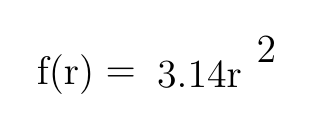
\begin{tikzpicture}
\node at (1.7,0) {{\Large 3.14r}};
\node at (2.55,0.32) {{\Large 2}};
\node at (0,0) {{\Large f(r)}};
\node at (0.7,0) {{\Large =}};
\end{tikzpicture}
\caption{Mathematical function for area of a circle}
\end{figure}

This function square the input value and multiply with 3.14.
Depending on the input value the output varies.

\begin{figure}[h!]
\centering
\begin{tikzpicture}
\draw [thick, ->] (0,1) -- (2,1);
\node at (.5,1.2) {r};
\draw [thick] (2,0) rectangle (7,2);
\node at (4.5,1) {3.14r};
\node at (5.1,1.2) {2};
\node at (4.5,2.3) {f(r)};
\draw [thick, ->] (7,1) -- (9,1);
\node at (8.5,1.2) {y};
\end{tikzpicture}
\caption{Blackbox representation of a function}
\end{figure}

As you can see in the above diagram, \texttt{r} is the input
and \texttt{y} is the output.  A function in Go can take input
arguments and perform actions and return values.  A simple
implementation of this function in Go looks like this.

\begin{lstlisting}[numbers=none]
func Area(r float64) float64 {
    return 3.14 * r * r
}
\end{lstlisting}

The function declaration starts with \texttt{func} keyword.  In the
above example, \texttt{Area} is the function name which can be later
used to call the function.  The arguments that can be received by this
function is given within brackets.  The line where function definition
started should end with an opening curly bracket.  The statements can
be written in the next line on wards until the closing curly bracket.

Here is a complete example with usage of the Area function.

\begin{lstlisting}[caption=Function usage]
package main

import "fmt"

// Area return the area of a circle for the given radius
func Area(r float64) float64 {
    return 3.14 * r * r
}

func main() {
    area := Area(5.0)
    fmt.Println(area)
}
\end{lstlisting}

In the above example, the \texttt{Area} function is called in line
number 11 with an argument of \texttt{5.0}.  We are using the short
variable declaration.  The type of the variable \texttt{area} will be
\texttt{float64} as the \texttt{Area} function returns with that type.

\subsection{Operators}

Programming languages use operators\index{operators} to simplify the
usage.  Operators behave more or less like functions.  More
specifically, operators combine operands to form expressions.  We have
already seen few operators
like \texttt{:=}, \texttt{=}, \texttt{+=}, \texttt{++}, \texttt{*},
\texttt{>} and \texttt{<}.

The \texttt{:=}, \texttt{=}, \texttt{+=} are assignment operators.
The \texttt{*} is the multiplication operator.  The \texttt{>}
and \texttt{<} are comparison operators.

Sometimes logical conditions should be checked to proceed with certain
steps.  Logical operators does these kind kind of checking.  Let's
say you want to check whether a particular value is divisible by 3
and 5.  You can do it like this.

\begin{lstlisting}[numbers=none]
if i%3 == 0 {
    if i%5 == 0 {
        // statements goes here
    }
}
\end{lstlisting}

The same thing can be achieved using conditional AND logical operator
(\texttt{\&\&}) like this.

\begin{lstlisting}[numbers=none]
if i%3 == 0 && i%5 == 0 {
    // statements goes here
}
\end{lstlisting}

Apart from the conditional AND, there are conditional OR (\texttt{||})
and NOT (\texttt{!}) logical operators.  We will see more about
operators in the next chapter.


\subsection{Slices}

Slice\index{slice} is a sequence of values of the same type.  In
computer science terminology, it's a homogeneous aggregate data type.
So, a slice can contain elements of only one type of data.  However,
it can hold a varying number of elements.  It can expand and shrink
the number of values.  \texttt{[]T} is a slice with elements of type
T.

The number of values in the slice is called the length of that slice.
The slice type \texttt{[]T} is a slice of type \texttt{T}.  Here is an
example slice of color names:

\begin{lstlisting}[numbers=none]
colors := []string{"Red", "Green", "Blue"}
\end{lstlisting}

In the above example, the length of slice is \texttt{3} and the slice
values are string data.  The \texttt{len} function gives the length of
slice.  See this complete example:

\begin{lstlisting}[caption=Printing slice values]
package main

import "fmt"

func main() {
    colors := []string{"Red", "Green", "Blue"}
    fmt.Println("Len:", len(colors))
    for i, v := range colors {
        fmt.Println(i, v)
    }
}
\end{lstlisting}

If you save the above program in a file named \texttt{colors.go} and
run it, you will get output like this:

\begin{lstlisting}[numbers=none]
$ go run colors.go
Len: 3
0 Red
1 Green
2 Blue
\end{lstlisting}

The \texttt{range}\index{range} clause loop over through elements in a
variety of data structures including slice and map.  Range gives index
and the value.  In the above example, the index is assigned
to \texttt{i} and value to \texttt{v} variables.  As you can see
above, each iteration change the value of \texttt{i} \& \texttt{v}.

If you are not interested in the index but just the value of string,
you can use blank identifier (variable).  In Go, underscore is
considered as blank identifier which you need not to define and you can
assign anything to it.  See the example written below to print each
string ignoring the index.

\begin{lstlisting}[caption=Range loop with index ignored]
package main

import "fmt"

func main() {
    colors := []string{"Red", "Green", "Blue"}
    fmt.Println("Len:", len(colors))
    for _, v := range colors {
        fmt.Println(v)
    }
}
\end{lstlisting}

If you just want to get the index without value, you can use just use
one variable to the left of range clause as give below.

\begin{lstlisting}[caption=Range loop without index]
package main

import "fmt"

func main() {
    colors := []string{"Red", "Green", "Blue"}
    fmt.Println("Len:", len(colors))
    for i := range colors {
        fmt.Println(i, colors[i])
    }
}
\end{lstlisting}

In the above example, we are accessing the value using the index
syntax: \texttt{colors[i]}.

\subsection{Maps}

Map\index{map} is another commonly used complex data structure in Go.
Map is an implementation of hash table which is available in many very
high level languages.  The data organized like key value pairs.  A
typical map type looks like this:

\begin{lstlisting}[numbers=none]
map[KeyType]ValueType
\end{lstlisting}

A \texttt{KeyType} can be any type that is comparable using the
comparison operators.  The \texttt{ValueType} can be any data type
including another map.  It is possible add any numbers of key value
pairs to the map.

Here is a map definition with some values initialized.

\begin{lstlisting}[numbers=none]
var fruits = map[string]int{
      "Apple":  45,
      "Mango":  24,
      "Orange": 34,
  }
\end{lstlisting}

To access a value corresponding to a key, you can use this syntax:

\begin{lstlisting}[numbers=none]
mangoCount := fruits["Mango"]
\end{lstlisting}

If the key doesn't exist, a zero value will be returned. For example, in the
below example, value of \texttt{pineappleCount} is going be \texttt{0}.

\begin{lstlisting}[numbers=none]
pineappleCount := fruits["Pineapple"]
\end{lstlisting}

More about maps will be explained in the data structure chapter.

\section{Exercises}

\textbf{Exercise 1:} Print multiples of 5 for all even numbers below 10

\textbf{Solution:}

This exercise requires getting all even numbers numbers below 10.  As
we we have seen above, a \texttt{for} loop can be used to get all
numbers.  Then \texttt{if} condition can be used with \texttt{\%}
operator to check whether the number is even or not.  The \texttt{\%}
operator given the gives the remainder and we can check it is zero or
not for modulus 2.  If the number is even use the \texttt{*} operator
to multiply with 5.

Here is the program.

\begin{lstlisting}[numbers=none]
package main

import "fmt"

func main() {
    for i := 1; i < 10; i++ {
        if i%2 == 0 {
            fmt.Println(i * 5)
        }
    }
}
\end{lstlisting}

\textbf{Exercise 2:} Create a function to reverse a string

\textbf{Solution:}

\begin{lstlisting}[numbers=none]
package main

import "fmt"

func Reverse(s string) string {
    var r string
    for _, c := range s {
        r = string(c) + r
    }
    return r
}

func main() {
    hw := "Hello, World!"
    rhw := Reverse(hw)
    fmt.Println(rhw)
}
\end{lstlisting}

\textbf{Exercise 3:} Find sum of all numbers below 50 completely divisible
by 2 or 3 (i.e., remainder 0).

Hint: The numbers completely divisible by 2 or 3 are 2, 3, 4, 6, 8, 9 ... 45,
46, 48.

\textbf{Solution:}

\begin{lstlisting}[numbers=none]
package main

import "fmt"

func main() {
    sum := 0
    for i := 1; i < 50; i++ {
        if i%2 == 0 {
            sum = sum + i
        } else {
            if i%3 == 0 {
                sum = sum + i
            }
        }
    }
    fmt.Println("Sum:", sum)
}
\end{lstlisting}

The logic can be simplified using a conditional OR operator.

\begin{lstlisting}[numbers=none]
package main

import "fmt"

func main() {
    sum := 0
    for i := 1; i < 50; i++ {
        if i%2 == 0 || i%3 == 0 {
            sum = sum + i
        }
    }
    fmt.Println("Sum:", sum)
}
\end{lstlisting}

\subsection{Additional Exercises}

Answers to these additional exercises are given in the Appendix A.

\textbf{Problem 1:} Write a function to check whether the first letter in a
given string is capital letters in English (A,B,C,D etc).

Hint: The signature of the function definition could be like this:
\texttt{func StartsCapital(s string) bool}.  If the function returns
\texttt{true}, the string passed starts with a capital letter.

\textbf{Problem 2:} Write a function to generate Fibonacci numbers below a
given value.

Hint: Suggested function signature: \texttt{func Fib(n int)}.  This
function can print the values.

\section*{Summary}

We began with a "hello world" program and briefly explained it. This chapter
then introduced a few basic topics in the Go programming language. We covered
data types, variables, comments, for loops, range clauses, if statements,
functions, operators, slices, and maps. The following chapters will explain the
fundamental concepts in more detail.
